
    


  \section{Casi di test e risultati}
    I test fatti sono di tipo \emph{oracolo} nel senso che l'output dell'algoritmo in ogni caso di test viene confrontato con il risultato che l'algoritmo dovrebbe fornire. 
    I test sono stati fatti su un laptop \emph{Hp Pavilion g6} con le seguenti caratteristiche:
    \begin{center}
      \begin{table}[!h]
      \centering
      \begin{tabular}{l|l}
	Microprocessore
      &
	Intel Core $i3-2330M$ da $2,2GHz$
      \\\hline
	Cache microprocessore
      &
	$3 MB$ di cache $L3$
      \\\hline
	Memoria
      &
	$DDR3$ da $6 GB$
    \end{tabular}
    \caption{Caratteristiche del calcolatore usato per i test.}
    \end{table}
  \end{center}

  \subsection{Casi di test sui file delle repository}
    I file usati in questo caso di test sono descritti in una sezione successiva \ref{repoDesc}.
    In seguito all'ascolto e alla visualizzazione della forma d'onda dei file, si nota che nessuno dei file contiene una apnea troppo lunga.
    La tabella \ref{esitoRepository} riporta nell'ordine: il nome del file, il tempo di esecuzione totale dell'algoritmo  e un errore approssimato nella localizzazione delle apnee.
    Il tempo di esecuzione dell'algoritmo \`e espresso come media dei tempi di esecuzione per secondo di segnale. 
\begin{table}
  \begin{tabular}{l l p{0.63\textwidth} }
  \hline
  File (.wav)						&Tempo			&Errore\\
\hline
  Coarse crackles					&$2ms$			&$0.4s$	nei veri positivi pi\`u un falso negativo		  \\
  Normal vesicular	 				&$14ms$			&$0.2s$	solo veri positivi					  \\
  Pleural friction					&$3ms$			&Il suono \`e troppo rumoroso e il sistema riconosce solo due pause respiratorie in modo corretto su quattro								  \\
  Inspiratory stridor					&$3ms$			&Il sistema riconosce l'inspirazione con una margine di errore di $0.4s$ ma confonde l'espirazione con una pausa perch\'e questa ha una intensit\`a molto bassa			  					  \\
  \hline
  \end{tabular}
  \caption{Esito dei test sui file delle repository}
  \label{esitoRepository}
\end{table}


\begin{comment}

/home/federico/tesi/Pleural friction.wav
0.0 - 0.5s: not breathing
0.5 - 9.6s: breathing
9.6 - 10.1s: not breathing
10.1 -  20.0s: breathing
_____***********************************************************************************************__**************************************************************************************************






/home/federico/tesi/Inspiratory stridor.wav

0.0 - 1.0s: not breathing
1.0 - 2.0s: breathing
2.0 - 3.6s: not breathing
3.6 - 5.s: breathing
5.0 - 6.2s: not breathing
6.2 - 7.8s: breathing
7.8 - 8.8s: not breathing
8.8 - 9.8s: breathing
9.8 - 10.2s: not breathing
10.2 - 10.8s: breathing
10.8 - 11.7s: not breathing
11.7 - 12.8s: breathing
12.8 - 14.4s: not breathing

__________**********________________**************____________******************_________***********___*******________************_______________




\end{comment}


\begin{comment}

tempo totale!

Normal Split Second Sound.wav 485 ms 
wheeze1.wav  45 ms 
stridor (1).wav  228 ms 
Normal Split S1.wav  18 ms 
Sibilo-Wheezing.wav  20 ms 
stridor.wav  36 ms 
wheeze.wav  220 ms 
vesicular.wav  231 ms 
crackle1.wav  76 ms 
\end{comment}



\begin{comment}
/home/federico/tesi/Coarse crackles.wav

0.0 - 1.0: not breathing
1.0s - 2.0s: breathing
2.0 - 3.3s: not breathing
3.3 - 4.0s: breathing
4.0 - 7.6s: not breathing
7.6 - 9.8s: not breathing
9.8 - 11.0s: breathing
11.0 - 12.5s: not breathing

__________**********_____________*******____________________________________**************________************_______________  





/home/federico/tesi/MurmureVescicolare-Normal vesicular.wav

0.0 - 0.9s: not breathing
0.9s - 2.0s: breathing
2.0 - 5.0s: not breathing
5.0 - 6.0s: breathing
6.0 - 6.2s: not breathing
6.2 - 7.0s: breathing
7.0 - 8.6s: not breathing
8.6 - 9.6s: breathing
9.6 - 12.6s: not breathing
_________***********______________________________**********__********________________**************______________________________

\end{comment}






\subsection{Caso di test di tolleranza al rumore bianco}
Il protagonista di questo caso di test \`e il file Normal vesicular.wav che contiene un suono respiratorio normale disturbato da un rumore leggero. A questo file aggiungiamo con Audacity del rumore bianco di intensit\`a crescente e valutiamo le prestazioni del sistema. Il file ha le seguenti caratteristiche:
\begin{itemize}
 \item 
    L'intensit\`a massima \`e circa $0.2dB$.
  \item
    L'intensit\`a media delle fasi inspiratorie \`e circa $0.08dB$.
  \item
    L'intensit\`a media delle fasi di pause respiratorie \`e circa $0.02dB$.
%   \item
%     Le fasi inspiratorie stimate ascoltando il file sono approssimativamente 
% 		      da $0.8s$ a $1.9s$, da $4.9s$ a $5.5s$ e da $8.5s$ a $9.2s$. Le fasi espiratorie sono approssimativamente localizzate 
% 		      da $1.9s$ a $2.2s$, da $6.0s$ a $6.6s$ e da $9.5s$ a $9.9s$ mentre le pause respiratorie sono localizzate 
%     da $0.0s$ a $0.8s$, $2.2s$ a $4.9s$, da $6.6s$ a $8.5s$ e da $9.9s$ a $13.0s$. 
%     Questi valori sono approssimativi e non \`e possibile ottenere valori pi\`u precisi se non si misura il flusso d'aria in modo diretto.
%     Il file si pu\`o rappresentare con la seguente sequenza 
%     
% 
\end{itemize}

L'intensit\`a del rumore aggiunto va da $0dB$ a $0.2dB$ con un incremento di $0.02dB$, quindi eseguiamo $11$ test. 
In nessun caso era presente una apnea troppo lunga e in nessun caso l'algoritmo ha rilevato la presenza di una apnea troppo lunga quindi dal punto di vista del riconoscimento di apnee troppo lunghe, l'algoritmo funziona in modo corretto. 
\`E comunque interessante valutare l'output dell'algoritmo con un maggior livello di dettaglio. 
La figura \ref{testNormalWhiteNoise} illustra una rappresentazione dell'output dell'algoritmo sui file di test e contiene un grafico per ogni file di input.
\begin{figure}
 \centering
 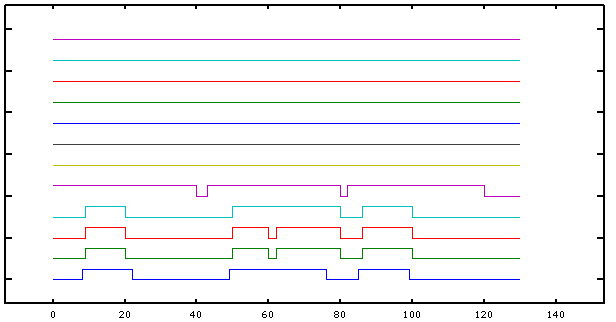
\includegraphics[width=0.9\textwidth]{./testWhiteNoise.png}
 % testWhiteNoise.png: 1366x768 pixel, 72dpi, 48.19x27.09 cm, bb=0 0 1366 768
  \caption{Risultati del test di tolleranza al rumore bianco.}
  \label{testNormalWhiteNoise}
\end{figure}

I valori sulle ascisse segnano il tempo in decimi di secondo.
I grafici contenuti nella figura dal basso verso l'alto escluso il primo sono relativi a file che hanno una quantit\`a di rumore crescente e mostrano quali parti dei rispettivi file vengono riconosciuti come respiro e quali parti vengono riconosciuti come apnea.
Invece il primo grafico in basso rappresenta il file originale in termini di fasi di respiro e fasi di pausa, stimate da un ascolto del file.
I valori di questo grafico sono approssimativi e non \`e possibile ottenere valori pi\`u precisi se non si misura il flusso d'aria in modo diretto.
Notiamo che gli ultimi $7$ grafici dal basso sono semplicemente dei segmenti di retta, questo perch\`e l'algoritmo riconosce l'intero file come respirazione cio\`e non riconosce alcuna pausa. 
Mentre nei primi $5$ grafici dal basso il segmento di retta pu\`o essere in basso ad indicare una pausa oppure in alto ad indicare la presenza di una inspirazione o di una espirazione.


% Nel grafico in figura \ref{graficoCasoDiTestRumoreBianco}, l'asse delle ascisse riporta la quantit\`a di rumore bianco aggiunto in termini di percentuale di decibel di rumore rispetto all'intensit\`a massima del respiro, mentre l'asse delle ordinate riporta l'errore calcolato in base a quanto detto nella sottosezione \ref{valutareOutput}.

\subsection{Caso di test di localizzazione di una apnea troppo lunga}
In questo caso di test prendiamo il file normal.wav reperito da \cite{SoundRepositories}, che contiene un respiro normale di un soggetto sano, lo concateniamo varie volte e aggiungiamo con Audacity una pausa respiratoria molto lunga. 
La pausa comincia all'istante $35s$ e termina all'istante $1m:17s$. 
La lunghezza totale del file \`e $1m:41s$.
Il sistema riconosce in modo corretto la pausa dall'istante $35s$ all'istante $1m:15s$.
L'allarme suona al tempo $63s$ cio\`e $30s$ dopo l'inizio della pausa, e questo \`e esattamente quello che ci aspettiamo.
Quindi possiamo dire che questo caso di test si \`e concluso con successo.



% \subsection{Casi di test della separazione dei suoni cardiaci da quelli respiratori}
% 
% \subsection{Casi di test di utilizzo della CPU}



\section{Descrizione dei file di respiro reperiti da \cite{SoundRepositories}}
\label{repoDesc}
    La tabella \ref{descrizioneRepo} seguente riporta una descrizione di alcuni dei file reperiti da \cite{SoundRepositories}. 
    Le colonne della tabella riportano nell'ordine: nome del file, durata del file, classificazione dei suoni respiratori contenuti nel file e infine frequenza di respirazione espressa in cicli di respirazione al secondo. 
    La frequenza di campionamento di tutti i file (espressa in numero di campioni al secondo) \`e di $8000 Hz$ e lo schema di respirazione \`e normale.
    
\begin{table}
  \begin{tabular}{l l l p{0.43\textwidth}}
  \hline
      Nome file 
    &
      Durata
    &
      Frequenza
    &
      Classificazione dei suoni respiratori
  \\\hline\\
      Coarse crackles.wav
    &
      $12s$
    &
      $25/60 Hz$
    &
      Normali e presenza di crackles
  \\
      Normal vesicular.wav
    &
      $13s$
    &
      $13.8/60 Hz$
    &
      Normali
 \\
      Inspiratory stridor.wav
    &
      $14s$
    &
      $21/60 Hz$
    &
      Normali e presenza di stridor durante la fase inspiratoria
  \\
      Pleural friction.wav
    &
      $20s$
    &
      $18/60 Hz$
    &
      Normali e presenza di frizione pleurica. Il suono \`e molto rumoroso e non \`ed \`e difficile distinguere le fasi respiratorie.
% \\
%       Coarse crackles.wav
%     &
%       $12s$
%     &
%       $25/60 Hz$
%     &
%       
% \\
%       Inspiratory stridor.wav
%     &
%       $14s$
%     &
%       $21/60 Hz$
%     &
      
  \\\hline
  \end{tabular}
  \caption{Descrizione dei file delle repository.}
  \label{descrizioneRepo}
\end{table}







% 
% \begin{table}
%   \begin{tabular}{p{0.47\textwidth}p{0.47\textwidth}}
%   \hline\\
%       Nome file 
%     &
%       Coarse crackles.wav
%   \\  
%       Durata
%     &
%       $12s$
%   \\
%       Frequenza di campionamento
%     &
%       $8000 Hz$
% %   \\
% %       Numero canali
% %     &
% %       Mono.
%   \\
%       Tipo di respirazione
%     &
%       Ritmo di respirazione normale. 
%   \\
%       Classificazione dei suoni
%     &
%       Suoni respiratori normali e presenza di crackles.
%   \\
%       Frequenza di respirazione
%     &
%        $\displaystyle\frac{25}{60}Hz$
%   \\\\\hline
%   \end{tabular}
%   \caption{Descrizione file Coarse crackles.wav.}
%   \label{Coarsecrackles}
% \end{table}
% 
% 
% \begin{table}
%   \begin{tabular}{p{0.47\textwidth}p{0.47\textwidth}}
%   \hline\\
%       Nome file 
%     &
%       Inspiratory stridor.wav
%   \\  
%       Durata
%     &
%       $14s$
%   \\
%       Frequenza di campionamento
%     &
%       $8000 Hz$
% %   \\
% %       Numero canali
% %     &
% %       Mono.
%   \\
%       Tipo di respirazione
%     &
%       Ritmo di respirazione normale. 
%   \\
%       Classificazione dei suoni
%     &
%       Suoni respiratori normali e presenza di stridor durante la fase inspiratoria.
%   \\
%       Frequenza di respirazione
%     &
%       $\displaystyle\frac{21}{60}Hz$
%  \\\\\hline
%   \end{tabular}
%   \caption{Descrizione file Inspiratory stridor.wav.}
%   \label{Inspiratorystridor}
% \end{table}
% 
% 
% 
% 
% 
% 
% 
% \begin{table}
%   \begin{tabular}{p{0.47\textwidth}p{0.47\textwidth}}
%   \hline\\
%       Nome file 
%     &
%       MurmureVescicolare-Normal vesicular.wav
%   \\  
%       Durata
%     &
%       $13s$
%   \\
%       Frequenza di campionamento
%     &
%       $8000 Hz$
% %   \\
% %       Numero canali
% %     &
% %       Mono.
%   \\
%       Tipo di respirazione
%     &
%       Ritmo di respirazione normale. 
%   \\
%       Classificazione dei suoni
%     &
%       Suoni respiratori normali.
%   \\
%       Frequenza di respirazione
%     &
%       $\displaystyle\frac{13.8}{60}Hz$
%  \\\\  \hline
%   \end{tabular}
%   \caption{Descrizione file MurmureVescicolare-Normal vesicular.wav}
%   \label{MurmureVescicolare}
% \end{table}
% 
% 
% 
% 
% 
% 
% 
% 
% 
% \begin{table}
%   \begin{tabular}{p{0.47\textwidth}p{0.47\textwidth}}
%   \hline\\
%       Nome file 
%     &
%       Pleural friction.wav
%   \\  
%       Durata
%     &
%       $13s$
%   \\
%       Frequenza di campionamento
%     &
%       $8000 Hz$
% %   \\
% %       Numero canali
% %     &
% %       Mono.
%   \\
%       Tipo di respirazione
%     &
%       Ritmo di respirazione normale. 
%   \\
%       Classificazione dei suoni
%     &
% 
%   \\
%       Frequenza di respirazione
%     &
%       $\displaystyle\frac{18}{60}Hz$
%  \\\\ \hline
%   \end{tabular}
%   \caption{Descrizione file Pleural friction.wav}
%   \label{Pleuralfriction}
% \end{table}
% 
% 
% 
% \begin{table}
%   \begin{tabular}{p{0.47\textwidth}p{0.47\textwidth}}
%   \hline\\
%       Nome file 
%     &
%       RantoliGrossolani-Coarse crackles.wav
%   \\  
%       Durata
%     &
%       $12s$
%   \\
%       Frequenza di campionamento
%     &
%       $8000 Hz$
% %   \\
% %       Numero canali
% %     &
% %       Mono.
%   \\
%       Tipo di respirazione
%     &
%       Ritmo di respirazione normale. 
%   \\
%       Classificazione dei suoni
%     &
%   \\
%       Frequenza di respirazione
%     &
%       $\displaystyle\frac{25}{60}Hz$
%  \\\\\hline
%   \end{tabular}
%   \caption{Descrizione file RantoliGrossolani-Coarse crackles.wav}
%   \label{RantoliGrossolani}
% \end{table}
% 
% 
% 
% 
% \begin{table}
%   \begin{tabular}{p{0.47\textwidth}p{0.47\textwidth}}
%   \hline\\
%       Nome file 
%     &
%       StridoreInspiratorio-Inspiratory stridor.wav
%   \\  
%       Durata
%     &
%       $14s$
%   \\
%       Frequenza di campionamento
%     &
%       $8000 Hz$
% %   \\
% %       Numero canali
% %     &
% %       Mono.
%   \\
%       Tipo di respirazione
%     &
%       Ritmo di respirazione normale. 
%   \\
%       Classificazione dei suoni
%     &
%   \\
%       Frequenza di respirazione
%     &
%       $\displaystyle\frac{21}{60}Hz$
%  \\\\  \hline
% 
%   \end{tabular}
%   \caption{Descrizione file StridoreInspiratorio-Inspiratory stridor.wav}
%   \label{StridoreInspiratorio}
% \end{table}
% 
% 
